% Options for packages loaded elsewhere
\PassOptionsToPackage{unicode}{hyperref}
\PassOptionsToPackage{hyphens}{url}
%
\documentclass[
]{article}
\usepackage{amsmath,amssymb}
\usepackage{iftex}
\ifPDFTeX
  \usepackage[T1]{fontenc}
  \usepackage[utf8]{inputenc}
  \usepackage{textcomp} % provide euro and other symbols
\else % if luatex or xetex
  \usepackage{unicode-math} % this also loads fontspec
  \defaultfontfeatures{Scale=MatchLowercase}
  \defaultfontfeatures[\rmfamily]{Ligatures=TeX,Scale=1}
\fi
\usepackage{lmodern}
\ifPDFTeX\else
  % xetex/luatex font selection
\fi
% Use upquote if available, for straight quotes in verbatim environments
\IfFileExists{upquote.sty}{\usepackage{upquote}}{}
\IfFileExists{microtype.sty}{% use microtype if available
  \usepackage[]{microtype}
  \UseMicrotypeSet[protrusion]{basicmath} % disable protrusion for tt fonts
}{}
\makeatletter
\@ifundefined{KOMAClassName}{% if non-KOMA class
  \IfFileExists{parskip.sty}{%
    \usepackage{parskip}
  }{% else
    \setlength{\parindent}{0pt}
    \setlength{\parskip}{6pt plus 2pt minus 1pt}}
}{% if KOMA class
  \KOMAoptions{parskip=half}}
\makeatother
\usepackage{xcolor}
\usepackage[margin=1in]{geometry}
\usepackage{color}
\usepackage{fancyvrb}
\newcommand{\VerbBar}{|}
\newcommand{\VERB}{\Verb[commandchars=\\\{\}]}
\DefineVerbatimEnvironment{Highlighting}{Verbatim}{commandchars=\\\{\}}
% Add ',fontsize=\small' for more characters per line
\usepackage{framed}
\definecolor{shadecolor}{RGB}{248,248,248}
\newenvironment{Shaded}{\begin{snugshade}}{\end{snugshade}}
\newcommand{\AlertTok}[1]{\textcolor[rgb]{0.94,0.16,0.16}{#1}}
\newcommand{\AnnotationTok}[1]{\textcolor[rgb]{0.56,0.35,0.01}{\textbf{\textit{#1}}}}
\newcommand{\AttributeTok}[1]{\textcolor[rgb]{0.13,0.29,0.53}{#1}}
\newcommand{\BaseNTok}[1]{\textcolor[rgb]{0.00,0.00,0.81}{#1}}
\newcommand{\BuiltInTok}[1]{#1}
\newcommand{\CharTok}[1]{\textcolor[rgb]{0.31,0.60,0.02}{#1}}
\newcommand{\CommentTok}[1]{\textcolor[rgb]{0.56,0.35,0.01}{\textit{#1}}}
\newcommand{\CommentVarTok}[1]{\textcolor[rgb]{0.56,0.35,0.01}{\textbf{\textit{#1}}}}
\newcommand{\ConstantTok}[1]{\textcolor[rgb]{0.56,0.35,0.01}{#1}}
\newcommand{\ControlFlowTok}[1]{\textcolor[rgb]{0.13,0.29,0.53}{\textbf{#1}}}
\newcommand{\DataTypeTok}[1]{\textcolor[rgb]{0.13,0.29,0.53}{#1}}
\newcommand{\DecValTok}[1]{\textcolor[rgb]{0.00,0.00,0.81}{#1}}
\newcommand{\DocumentationTok}[1]{\textcolor[rgb]{0.56,0.35,0.01}{\textbf{\textit{#1}}}}
\newcommand{\ErrorTok}[1]{\textcolor[rgb]{0.64,0.00,0.00}{\textbf{#1}}}
\newcommand{\ExtensionTok}[1]{#1}
\newcommand{\FloatTok}[1]{\textcolor[rgb]{0.00,0.00,0.81}{#1}}
\newcommand{\FunctionTok}[1]{\textcolor[rgb]{0.13,0.29,0.53}{\textbf{#1}}}
\newcommand{\ImportTok}[1]{#1}
\newcommand{\InformationTok}[1]{\textcolor[rgb]{0.56,0.35,0.01}{\textbf{\textit{#1}}}}
\newcommand{\KeywordTok}[1]{\textcolor[rgb]{0.13,0.29,0.53}{\textbf{#1}}}
\newcommand{\NormalTok}[1]{#1}
\newcommand{\OperatorTok}[1]{\textcolor[rgb]{0.81,0.36,0.00}{\textbf{#1}}}
\newcommand{\OtherTok}[1]{\textcolor[rgb]{0.56,0.35,0.01}{#1}}
\newcommand{\PreprocessorTok}[1]{\textcolor[rgb]{0.56,0.35,0.01}{\textit{#1}}}
\newcommand{\RegionMarkerTok}[1]{#1}
\newcommand{\SpecialCharTok}[1]{\textcolor[rgb]{0.81,0.36,0.00}{\textbf{#1}}}
\newcommand{\SpecialStringTok}[1]{\textcolor[rgb]{0.31,0.60,0.02}{#1}}
\newcommand{\StringTok}[1]{\textcolor[rgb]{0.31,0.60,0.02}{#1}}
\newcommand{\VariableTok}[1]{\textcolor[rgb]{0.00,0.00,0.00}{#1}}
\newcommand{\VerbatimStringTok}[1]{\textcolor[rgb]{0.31,0.60,0.02}{#1}}
\newcommand{\WarningTok}[1]{\textcolor[rgb]{0.56,0.35,0.01}{\textbf{\textit{#1}}}}
\usepackage{graphicx}
\makeatletter
\def\maxwidth{\ifdim\Gin@nat@width>\linewidth\linewidth\else\Gin@nat@width\fi}
\def\maxheight{\ifdim\Gin@nat@height>\textheight\textheight\else\Gin@nat@height\fi}
\makeatother
% Scale images if necessary, so that they will not overflow the page
% margins by default, and it is still possible to overwrite the defaults
% using explicit options in \includegraphics[width, height, ...]{}
\setkeys{Gin}{width=\maxwidth,height=\maxheight,keepaspectratio}
% Set default figure placement to htbp
\makeatletter
\def\fps@figure{htbp}
\makeatother
\setlength{\emergencystretch}{3em} % prevent overfull lines
\providecommand{\tightlist}{%
  \setlength{\itemsep}{0pt}\setlength{\parskip}{0pt}}
\setcounter{secnumdepth}{-\maxdimen} % remove section numbering
\ifLuaTeX
  \usepackage{selnolig}  % disable illegal ligatures
\fi
\IfFileExists{bookmark.sty}{\usepackage{bookmark}}{\usepackage{hyperref}}
\IfFileExists{xurl.sty}{\usepackage{xurl}}{} % add URL line breaks if available
\urlstyle{same}
\hypersetup{
  pdftitle={HUDM6052 Psychometric II Homework\_03},
  pdfauthor={Chenguang Pan (cp3280@tc.columbia.edu)},
  hidelinks,
  pdfcreator={LaTeX via pandoc}}

\title{HUDM6052 Psychometric II Homework\_03}
\author{Chenguang Pan
(\href{mailto:cp3280@tc.columbia.edu}{\nolinkurl{cp3280@tc.columbia.edu}})}
\date{2023-10-26}

\begin{document}
\maketitle

\setcounter{tocdepth}{4}
\tableofcontents

\hypertarget{q1}{%
\subsection{Q1}\label{q1}}

\emph{Using the item parameters given in the Table\ldots{}}

\textbf{My Solution:}

\begin{Shaded}
\begin{Highlighting}[]
\SpecialCharTok{\textgreater{}} \CommentTok{\# write the corresponding information function}
\ErrorTok{\textgreater{}}\NormalTok{ iif }\OtherTok{\textless{}{-}} \ControlFlowTok{function}\NormalTok{(theta, a, b)\{}
\SpecialCharTok{+}   \CommentTok{\# get the logit}
\SpecialCharTok{+}\NormalTok{   Z }\OtherTok{\textless{}{-}}\NormalTok{ a}\SpecialCharTok{*}\NormalTok{(theta}\SpecialCharTok{{-}}\NormalTok{b)}
\SpecialCharTok{+}   \CommentTok{\# get the probability}
\SpecialCharTok{+}\NormalTok{   out }\OtherTok{\textless{}{-}} \DecValTok{1}\SpecialCharTok{/}\NormalTok{(}\DecValTok{1} \SpecialCharTok{+} \FunctionTok{exp}\NormalTok{(}\SpecialCharTok{{-}}\NormalTok{Z))}
\SpecialCharTok{+}\NormalTok{   info }\OtherTok{\textless{}{-}}\NormalTok{ out}\SpecialCharTok{*}\NormalTok{(}\DecValTok{1}\SpecialCharTok{{-}}\NormalTok{out)}\SpecialCharTok{*}\NormalTok{(a}\SpecialCharTok{\^{}}\DecValTok{2}\NormalTok{)}
\SpecialCharTok{+}   \FunctionTok{return}\NormalTok{(info)}
\SpecialCharTok{+}\NormalTok{ \}}
\SpecialCharTok{\textgreater{}} 
\ErrorTok{\textgreater{}} \CommentTok{\# set the ability range}
\ErrorTok{\textgreater{}}\NormalTok{ theta }\OtherTok{\textless{}{-}} \FunctionTok{seq}\NormalTok{(}\SpecialCharTok{{-}}\DecValTok{3}\NormalTok{,}\DecValTok{3}\NormalTok{, }\AttributeTok{by=}\FloatTok{0.5}\NormalTok{)}
\SpecialCharTok{\textgreater{}} \CommentTok{\# set the item parameters}
\ErrorTok{\textgreater{}}\NormalTok{ a }\OtherTok{\textless{}{-}} \FunctionTok{c}\NormalTok{(}\DecValTok{2}\NormalTok{, }\FloatTok{1.5}\NormalTok{, }\FloatTok{1.5}\NormalTok{, }\FloatTok{1.5}\NormalTok{, }\DecValTok{2}\NormalTok{)}
\SpecialCharTok{\textgreater{}}\NormalTok{ b }\OtherTok{\textless{}{-}} \FunctionTok{c}\NormalTok{(}\SpecialCharTok{{-}}\DecValTok{1}\NormalTok{, }\SpecialCharTok{{-}}\FloatTok{0.5}\NormalTok{, }\DecValTok{0}\NormalTok{, }\FloatTok{0.5}\NormalTok{, }\DecValTok{1}\NormalTok{)}
\SpecialCharTok{\textgreater{}} \CommentTok{\# define the color}
\ErrorTok{\textgreater{}}\NormalTok{ color\_set }\OtherTok{\textless{}{-}} \FunctionTok{c}\NormalTok{(}\StringTok{"red"}\NormalTok{, }\StringTok{"green"}\NormalTok{, }\StringTok{"blue"}\NormalTok{,}\StringTok{"violet"}\NormalTok{,}\StringTok{"black"}\NormalTok{)}
\SpecialCharTok{\textgreater{}} 
\ErrorTok{\textgreater{}} \CommentTok{\# plot the item information function}
\ErrorTok{\textgreater{}}\NormalTok{ info\_out }\OtherTok{\textless{}{-}} \FunctionTok{iif}\NormalTok{(theta, a[}\DecValTok{1}\NormalTok{], b[}\DecValTok{1}\NormalTok{])}
\SpecialCharTok{\textgreater{}} \CommentTok{\# create a vector to sum up all the information function}
\ErrorTok{\textgreater{}}\NormalTok{ test\_info }\OtherTok{\textless{}{-}}\NormalTok{ info\_out}
\SpecialCharTok{\textgreater{}} 
\ErrorTok{\textgreater{}} \CommentTok{\# initialize the plot by plotting the first item}
\ErrorTok{\textgreater{}} \FunctionTok{plot}\NormalTok{(theta, info\_out,}\AttributeTok{type =} \StringTok{"l"}\NormalTok{, }\AttributeTok{col=}\NormalTok{color\_set[}\DecValTok{1}\NormalTok{],}
\SpecialCharTok{+}      \AttributeTok{main =} \StringTok{"Item/Test Information and SEs"}\NormalTok{,}
\SpecialCharTok{+}      \AttributeTok{xlab =} \StringTok{"Ability"}\NormalTok{, }\AttributeTok{ylab =} \StringTok{"information"}\NormalTok{,}
\SpecialCharTok{+}      \AttributeTok{ylim =} \FunctionTok{c}\NormalTok{(}\DecValTok{0}\NormalTok{,}\DecValTok{3}\NormalTok{))}
\SpecialCharTok{\textgreater{}} \FunctionTok{grid}\NormalTok{()}
\SpecialCharTok{\textgreater{}} 
\ErrorTok{\textgreater{}} \CommentTok{\# plot the rest item using a for loop}
\ErrorTok{\textgreater{}} \ControlFlowTok{for}\NormalTok{ (i }\ControlFlowTok{in} \DecValTok{2}\SpecialCharTok{:}\DecValTok{5}\NormalTok{) \{}
\SpecialCharTok{+}\NormalTok{   info\_out\_i }\OtherTok{\textless{}{-}} \FunctionTok{iif}\NormalTok{(theta,a[i],b[i])}
\SpecialCharTok{+}   \FunctionTok{lines}\NormalTok{(theta, info\_out\_i, }\AttributeTok{type =}\StringTok{"l"}\NormalTok{, }\AttributeTok{col=}\NormalTok{color\_set[i])}
\SpecialCharTok{+}\NormalTok{   test\_info }\OtherTok{\textless{}{-}}\NormalTok{ test\_info }\SpecialCharTok{+}\NormalTok{info\_out\_i}
\SpecialCharTok{+}\NormalTok{ \}}
\SpecialCharTok{\textgreater{}} 
\ErrorTok{\textgreater{}} \CommentTok{\# draw the test information function}
\ErrorTok{\textgreater{}} \FunctionTok{lines}\NormalTok{(theta, test\_info, }\AttributeTok{type =} \StringTok{"l"}\NormalTok{, }\AttributeTok{col=}\StringTok{"gray"}\NormalTok{)}
\SpecialCharTok{\textgreater{}} \CommentTok{\# plot the SE }
\ErrorTok{\textgreater{}}\NormalTok{ SE }\OtherTok{\textless{}{-}} \FunctionTok{c}\NormalTok{()}
\SpecialCharTok{\textgreater{}} \ControlFlowTok{for}\NormalTok{ (j }\ControlFlowTok{in} \DecValTok{1}\SpecialCharTok{:}\FunctionTok{length}\NormalTok{(theta)) \{}
\SpecialCharTok{+}\NormalTok{   se\_j }\OtherTok{\textless{}{-}} \DecValTok{1}\SpecialCharTok{/}\FunctionTok{sqrt}\NormalTok{(}\FunctionTok{sum}\NormalTok{(}\FunctionTok{iif}\NormalTok{(theta[j],a,b)))}
\SpecialCharTok{+}\NormalTok{   SE[j] }\OtherTok{\textless{}{-}}\NormalTok{ se\_j}
\SpecialCharTok{+}\NormalTok{ \}}
\SpecialCharTok{\textgreater{}} \FunctionTok{lines}\NormalTok{(theta, SE, }\AttributeTok{type =} \StringTok{"l"}\NormalTok{, }\AttributeTok{col=}\StringTok{"pink"}\NormalTok{)}
\SpecialCharTok{\textgreater{}} 
\ErrorTok{\textgreater{}} \CommentTok{\# add a legend}
\ErrorTok{\textgreater{}} \FunctionTok{legend}\NormalTok{(}\StringTok{\textquotesingle{}topright\textquotesingle{}}\NormalTok{,}\AttributeTok{inset=}\FloatTok{0.05}\NormalTok{,}\FunctionTok{c}\NormalTok{(}\StringTok{"item 1"}\NormalTok{,}\StringTok{"item 2"}\NormalTok{,}\StringTok{"item 3"}\NormalTok{,}\StringTok{"item 4"}\NormalTok{,}\StringTok{"item 5"}\NormalTok{,}
\SpecialCharTok{+}                               \StringTok{"test information"}\NormalTok{,}\StringTok{"SE"}\NormalTok{),}
\SpecialCharTok{+}        \AttributeTok{lty=}\DecValTok{1}\NormalTok{,}\AttributeTok{col=}\FunctionTok{c}\NormalTok{(}\StringTok{"red"}\NormalTok{, }\StringTok{"green"}\NormalTok{,}\StringTok{"blue"}\NormalTok{,}\StringTok{"violet"}\NormalTok{,}\StringTok{"black"}\NormalTok{,}\StringTok{"gray"}\NormalTok{,}\StringTok{"pink"}\NormalTok{),}
\SpecialCharTok{+}        \AttributeTok{title=}\StringTok{"Line Type"}\NormalTok{, }\AttributeTok{cex =} \FloatTok{0.5}\NormalTok{)}
\end{Highlighting}
\end{Shaded}

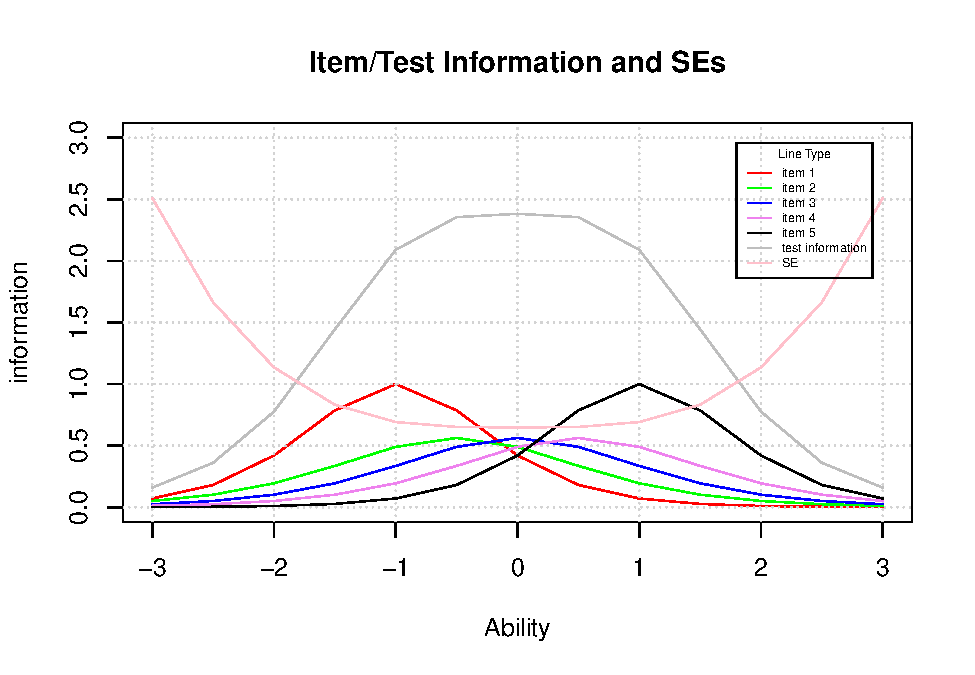
\includegraphics{Assignment_3_files/figure-latex/unnamed-chunk-1-1.pdf}

\hypertarget{q2.a}{%
\subsection{Q2.a}\label{q2.a}}

\emph{a. For each of the six items given in the Table below\ldots{}}

\textbf{My Solution:}\\
The maximum value of a 3PL's information function is at
\[\theta_{max}=\beta_i + \frac{1}{a_i}log[\frac{1+\sqrt{1+8c_i}}{2}].\]\\
Therefore, I write a function to get the optimal \(\theta_{max}\) first.
And then send this value together with the parameters into the
information function for 3PL model to get the results.

\begin{Shaded}
\begin{Highlighting}[]
\SpecialCharTok{\textgreater{}} \CommentTok{\# write a function to get the theta\_max}
\ErrorTok{\textgreater{}}\NormalTok{ get\_theta }\OtherTok{\textless{}{-}} \ControlFlowTok{function}\NormalTok{(a,b,c)\{}
\SpecialCharTok{+}\NormalTok{   out }\OtherTok{\textless{}{-}}\NormalTok{ b }\SpecialCharTok{+} \FunctionTok{log}\NormalTok{(}\FloatTok{0.5+0.5}\SpecialCharTok{*}\FunctionTok{sqrt}\NormalTok{(}\DecValTok{1}\SpecialCharTok{+}\DecValTok{8}\SpecialCharTok{*}\NormalTok{c))}\SpecialCharTok{/}\NormalTok{a}
\SpecialCharTok{+}   \FunctionTok{return}\NormalTok{(out)}
\SpecialCharTok{+}\NormalTok{ \}}
\SpecialCharTok{\textgreater{}} 
\ErrorTok{\textgreater{}} \CommentTok{\# write the 3pl information function}
\ErrorTok{\textgreater{}}\NormalTok{ iif\_3pl }\OtherTok{\textless{}{-}} \ControlFlowTok{function}\NormalTok{(theta, a, b, c)\{}
\SpecialCharTok{+}\NormalTok{   z }\OtherTok{\textless{}{-}}\NormalTok{ a}\SpecialCharTok{*}\NormalTok{(theta }\SpecialCharTok{{-}}\NormalTok{ b)}
\SpecialCharTok{+}\NormalTok{   p }\OtherTok{\textless{}{-}}\NormalTok{ c }\SpecialCharTok{+}\NormalTok{ (}\DecValTok{1}\SpecialCharTok{{-}}\NormalTok{c)}\SpecialCharTok{/}\NormalTok{(}\DecValTok{1}\SpecialCharTok{+}\FunctionTok{exp}\NormalTok{(}\SpecialCharTok{{-}}\NormalTok{z))}
\SpecialCharTok{+}\NormalTok{   p\_star }\OtherTok{\textless{}{-}} \DecValTok{1}\SpecialCharTok{/}\NormalTok{(}\DecValTok{1} \SpecialCharTok{+} \FunctionTok{exp}\NormalTok{(}\SpecialCharTok{{-}}\NormalTok{z))}
\SpecialCharTok{+}\NormalTok{   I }\OtherTok{\textless{}{-}}\NormalTok{ (a}\SpecialCharTok{\^{}}\DecValTok{2}\NormalTok{)}\SpecialCharTok{*}\NormalTok{p}\SpecialCharTok{*}\NormalTok{(}\DecValTok{1}\SpecialCharTok{{-}}\NormalTok{p)}\SpecialCharTok{*}\NormalTok{(p\_star}\SpecialCharTok{/}\NormalTok{p)}\SpecialCharTok{\^{}}\DecValTok{2}
\SpecialCharTok{+}   \FunctionTok{return}\NormalTok{(I)}
\SpecialCharTok{+}\NormalTok{ \}}
\end{Highlighting}
\end{Shaded}

Next, plug the given paramters into the functions to get the results.

\begin{Shaded}
\begin{Highlighting}[]
\SpecialCharTok{\textgreater{}} \CommentTok{\# load the given parameters vectors}
\ErrorTok{\textgreater{}}\NormalTok{ b }\OtherTok{\textless{}{-}} \FunctionTok{c}\NormalTok{(}\DecValTok{1}\NormalTok{,}\DecValTok{1}\NormalTok{,}\DecValTok{1}\NormalTok{,}\SpecialCharTok{{-}}\FloatTok{1.5}\NormalTok{,}\SpecialCharTok{{-}}\FloatTok{0.5}\NormalTok{,}\FloatTok{0.5}\NormalTok{)}
\SpecialCharTok{\textgreater{}}\NormalTok{ a }\OtherTok{\textless{}{-}} \FunctionTok{c}\NormalTok{(}\FloatTok{1.8}\NormalTok{,}\FloatTok{0.8}\NormalTok{,}\FloatTok{1.8}\NormalTok{,}\FloatTok{1.8}\NormalTok{,}\FloatTok{1.2}\NormalTok{,}\FloatTok{0.4}\NormalTok{)}
\SpecialCharTok{\textgreater{}}\NormalTok{ c }\OtherTok{\textless{}{-}} \FunctionTok{c}\NormalTok{(}\DecValTok{0}\NormalTok{,}\DecValTok{0}\NormalTok{,}\FloatTok{0.25}\NormalTok{,}\DecValTok{0}\NormalTok{,}\FloatTok{0.1}\NormalTok{,}\FloatTok{0.15}\NormalTok{)}
\SpecialCharTok{\textgreater{}} 
\ErrorTok{\textgreater{}} \CommentTok{\# using a for loop to get all the required values}
\ErrorTok{\textgreater{}}\NormalTok{ theta\_vec }\OtherTok{\textless{}{-}} \FunctionTok{c}\NormalTok{()}
\SpecialCharTok{\textgreater{}}\NormalTok{ info\_vec }\OtherTok{\textless{}{-}} \FunctionTok{c}\NormalTok{()}
\SpecialCharTok{\textgreater{}} \ControlFlowTok{for}\NormalTok{ (i }\ControlFlowTok{in} \DecValTok{1}\SpecialCharTok{:}\FunctionTok{length}\NormalTok{(b)) \{}
\SpecialCharTok{+}   \CommentTok{\# get the optimal theta value}
\SpecialCharTok{+}\NormalTok{   theta\_max }\OtherTok{\textless{}{-}} \FunctionTok{get\_theta}\NormalTok{(}\AttributeTok{a =}\NormalTok{ a[i],}\AttributeTok{b =}\NormalTok{ b[i],}\AttributeTok{c =}\NormalTok{ c[i])}
\SpecialCharTok{+}\NormalTok{   theta\_vec[i] }\OtherTok{\textless{}{-}}\NormalTok{ theta\_max}
\SpecialCharTok{+}   \CommentTok{\# get the maximum value of information of item i}
\SpecialCharTok{+}\NormalTok{   info\_max }\OtherTok{\textless{}{-}} \FunctionTok{iif\_3pl}\NormalTok{(}\AttributeTok{theta =}\NormalTok{ theta\_max,}\AttributeTok{a =}\NormalTok{ a[i],}\AttributeTok{b =}\NormalTok{ b[i],}\AttributeTok{c =}\NormalTok{ c[i])}
\SpecialCharTok{+}\NormalTok{   info\_vec[i] }\OtherTok{\textless{}{-}}\NormalTok{ info\_max}
\SpecialCharTok{+}\NormalTok{ \}}
\SpecialCharTok{\textgreater{}} 
\ErrorTok{\textgreater{}} \CommentTok{\# Merge all the values as a dataframe}
\ErrorTok{\textgreater{}}\NormalTok{ df\_out }\OtherTok{\textless{}{-}} \FunctionTok{data.frame}\NormalTok{(}
\SpecialCharTok{+}   \AttributeTok{item =} \FunctionTok{seq}\NormalTok{(}\DecValTok{1}\NormalTok{,}\DecValTok{6}\NormalTok{),}
\SpecialCharTok{+}   \AttributeTok{theta\_max =}\NormalTok{ theta\_vec,}
\SpecialCharTok{+}   \AttributeTok{info\_max =}\NormalTok{ info\_vec}
\SpecialCharTok{+}\NormalTok{ )}
\SpecialCharTok{\textgreater{}} 
\ErrorTok{\textgreater{}}\NormalTok{ df\_out}
\NormalTok{  item  theta\_max   info\_max}
\DecValTok{1}    \DecValTok{1}  \FloatTok{1.0000000} \FloatTok{0.81000000}
\DecValTok{2}    \DecValTok{2}  \FloatTok{1.0000000} \FloatTok{0.16000000}
\DecValTok{3}    \DecValTok{3}  \FloatTok{1.1732808} \FloatTok{0.50122974}
\DecValTok{4}    \DecValTok{4} \SpecialCharTok{{-}}\FloatTok{1.5000000} \FloatTok{0.81000000}
\DecValTok{5}    \DecValTok{5} \SpecialCharTok{{-}}\FloatTok{0.3685794} \FloatTok{0.29665631}
\DecValTok{6}    \DecValTok{6}  \FloatTok{1.0410421} \FloatTok{0.02998276}
\end{Highlighting}
\end{Shaded}

The maximum values of information and corresponding \(\theta s\) are
shown at end of the code chunk above.

\hypertarget{q2.b}{%
\subsection{Q2.b}\label{q2.b}}

\emph{b. Which item would you choose to make up a two-item\ldots{}}

\textbf{My Solution:}\\
I will choose the \texttt{item\ 1} and \texttt{item\ 2} to make a
two-item test since they have the maximum information at the
\(\theta = 1.0\), which means this test can more accurately measure this
given test-taker's ability. The test information at \(\theta = 1.0\) is
\[0.81+0.16=0.97.\]

\hypertarget{q3.a}{%
\subsection{Q3.a}\label{q3.a}}

\emph{a. Determine the standard error of the estimate\ldots{}}

\textbf{My Solution:}

\begin{Shaded}
\begin{Highlighting}[]
\SpecialCharTok{\textgreater{}} \CommentTok{\# load the given paramters}
\ErrorTok{\textgreater{}}\NormalTok{ a }\OtherTok{\textless{}{-}} \FunctionTok{c}\NormalTok{(}\DecValTok{1}\NormalTok{,}\DecValTok{1}\NormalTok{,}\DecValTok{2}\NormalTok{,}\DecValTok{2}\NormalTok{)}
\SpecialCharTok{\textgreater{}}\NormalTok{ b }\OtherTok{\textless{}{-}} \FunctionTok{c}\NormalTok{(}\DecValTok{0}\NormalTok{,}\DecValTok{1}\NormalTok{,}\DecValTok{1}\NormalTok{,}\FloatTok{1.5}\NormalTok{)}
\SpecialCharTok{\textgreater{}}\NormalTok{ theta }\OtherTok{\textless{}{-}} \FloatTok{1.5}
\SpecialCharTok{\textgreater{}} 
\ErrorTok{\textgreater{}} \CommentTok{\# using the information function created in the Q1 to get the }
\ErrorTok{\textgreater{}} \CommentTok{\# vector of information at the theta=1.5 for each item}
\ErrorTok{\textgreater{}}\NormalTok{ info\_vec }\OtherTok{\textless{}{-}} \FunctionTok{iif}\NormalTok{(}\AttributeTok{theta=}\FloatTok{1.5}\NormalTok{, a, b)}
\SpecialCharTok{\textgreater{}} 
\ErrorTok{\textgreater{}} \CommentTok{\# get the SE}
\ErrorTok{\textgreater{}}\NormalTok{ SE\_j }\OtherTok{\textless{}{-}} \DecValTok{1}\SpecialCharTok{/}\FunctionTok{sqrt}\NormalTok{(}\FunctionTok{sum}\NormalTok{(info\_vec))}
\SpecialCharTok{\textgreater{}}\NormalTok{ SE\_j}
\NormalTok{[}\DecValTok{1}\NormalTok{] }\FloatTok{0.6787507}
\end{Highlighting}
\end{Shaded}

Therefore, the SE for the test-taker with estimated trait \(\theta=1.5\)
is 0.679.

\hypertarget{q3.b}{%
\subsection{Q3.b}\label{q3.b}}

\emph{b. Construct a 95\% confidence interval for\ldots{}}

\textbf{My Solution:}\\
The 95\% confidence interval of the estimated \(\theta=1.5\) is
\[95\%CI = 1.5\pm 1.96\times 0.679.\]\\
Therefore, \(95\%CI\) is \([.169, 2.831].\)

\hypertarget{q4}{%
\subsection{Q4}\label{q4}}

\emph{Fit 3PL model to the dataset\ldots{}}

\textbf{My Solution:}\\
For estimating the 3PL model,

\begin{Shaded}
\begin{Highlighting}[]
\SpecialCharTok{\textgreater{}} \CommentTok{\# load the data}
\ErrorTok{\textgreater{}}\NormalTok{ widths }\OtherTok{\textless{}{-}} \FunctionTok{c}\NormalTok{(}\DecValTok{4}\NormalTok{, }\FunctionTok{rep}\NormalTok{(}\DecValTok{1}\NormalTok{,}\DecValTok{40}\NormalTok{))}
\SpecialCharTok{\textgreater{}}\NormalTok{ df }\OtherTok{\textless{}{-}} \FunctionTok{read.fwf}\NormalTok{(}\StringTok{"\textasciitilde{}/Desktop/PhD\_Learning/HUDM6052 Psychometric II/HUDM6052\_Psychometic\_II/Assignment 3/sample{-}1.dat"}\NormalTok{, }\AttributeTok{widths =}\NormalTok{ widths,}
\SpecialCharTok{+}                \AttributeTok{header =}\NormalTok{ F, }\AttributeTok{stringsAsFactors=}\NormalTok{F)}
\SpecialCharTok{\textgreater{}} 
\ErrorTok{\textgreater{}} \CommentTok{\# rename the columns}
\ErrorTok{\textgreater{}}\NormalTok{ items\_name }\OtherTok{\textless{}{-}} \FunctionTok{paste0}\NormalTok{(}\StringTok{"item\_"}\NormalTok{, }\FunctionTok{seq}\NormalTok{(}\DecValTok{1}\NormalTok{,}\DecValTok{40}\NormalTok{))}
\SpecialCharTok{\textgreater{}}\NormalTok{ col\_names }\OtherTok{\textless{}{-}} \FunctionTok{c}\NormalTok{(}\StringTok{"ID"}\NormalTok{, items\_name)}
\SpecialCharTok{\textgreater{}} \FunctionTok{names}\NormalTok{(df) }\OtherTok{\textless{}{-}}\NormalTok{ col\_names}
\SpecialCharTok{\textgreater{}} 
\ErrorTok{\textgreater{}} \CommentTok{\# fit the 3PL model through MIRT package}
\ErrorTok{\textgreater{}} \FunctionTok{library}\NormalTok{(mirt)}
\SpecialCharTok{\textgreater{}} \CommentTok{\# step 1: specify the model, 40 items load on one factor}
\ErrorTok{\textgreater{}} \CommentTok{\#         set a prior distribution for the pseudo{-}guessing parameter to}
\ErrorTok{\textgreater{}} \CommentTok{\#         reduce problems of estimation convergence}
\ErrorTok{\textgreater{}}\NormalTok{ spec }\OtherTok{\textless{}{-}} \StringTok{\textquotesingle{}F = 1{-}40}
\StringTok{+ PRIOR = (1{-}40,g,norm, {-}1.1,2)\textquotesingle{}}
\SpecialCharTok{\textgreater{}} 
\ErrorTok{\textgreater{}} \CommentTok{\# step 2: fit the model}
\ErrorTok{\textgreater{}}\NormalTok{ mod\_3pl }\OtherTok{\textless{}{-}} \FunctionTok{mirt}\NormalTok{(df[,}\SpecialCharTok{{-}}\DecValTok{1}\NormalTok{], }\AttributeTok{model=}\NormalTok{spec,}\AttributeTok{itemtype =} \StringTok{"3PL"}\NormalTok{, }\AttributeTok{SE=}\NormalTok{T)}
\NormalTok{Iteration}\SpecialCharTok{:} \DecValTok{1}\NormalTok{, Log}\SpecialCharTok{{-}}\NormalTok{Lik}\SpecialCharTok{:} \SpecialCharTok{{-}}\FloatTok{11855.215}\NormalTok{, Max}\SpecialCharTok{{-}}\NormalTok{Change}\SpecialCharTok{:} \FloatTok{1.43351}\NormalTok{Iteration}\SpecialCharTok{:} \DecValTok{2}\NormalTok{, Log}\SpecialCharTok{{-}}\NormalTok{Lik}\SpecialCharTok{:} \SpecialCharTok{{-}}\FloatTok{11673.391}\NormalTok{, Max}\SpecialCharTok{{-}}\NormalTok{Change}\SpecialCharTok{:} \FloatTok{0.90335}\NormalTok{Iteration}\SpecialCharTok{:} \DecValTok{3}\NormalTok{, Log}\SpecialCharTok{{-}}\NormalTok{Lik}\SpecialCharTok{:} \SpecialCharTok{{-}}\FloatTok{11641.104}\NormalTok{, Max}\SpecialCharTok{{-}}\NormalTok{Change}\SpecialCharTok{:} \FloatTok{0.99048}\NormalTok{Iteration}\SpecialCharTok{:} \DecValTok{4}\NormalTok{, Log}\SpecialCharTok{{-}}\NormalTok{Lik}\SpecialCharTok{:} \SpecialCharTok{{-}}\FloatTok{11624.617}\NormalTok{, Max}\SpecialCharTok{{-}}\NormalTok{Change}\SpecialCharTok{:} \FloatTok{0.72041}\NormalTok{Iteration}\SpecialCharTok{:} \DecValTok{5}\NormalTok{, Log}\SpecialCharTok{{-}}\NormalTok{Lik}\SpecialCharTok{:} \SpecialCharTok{{-}}\FloatTok{11614.499}\NormalTok{, Max}\SpecialCharTok{{-}}\NormalTok{Change}\SpecialCharTok{:} \FloatTok{0.28020}\NormalTok{Iteration}\SpecialCharTok{:} \DecValTok{6}\NormalTok{, Log}\SpecialCharTok{{-}}\NormalTok{Lik}\SpecialCharTok{:} \SpecialCharTok{{-}}\FloatTok{11608.099}\NormalTok{, Max}\SpecialCharTok{{-}}\NormalTok{Change}\SpecialCharTok{:} \FloatTok{0.17815}\NormalTok{Iteration}\SpecialCharTok{:} \DecValTok{7}\NormalTok{, Log}\SpecialCharTok{{-}}\NormalTok{Lik}\SpecialCharTok{:} \SpecialCharTok{{-}}\FloatTok{11603.682}\NormalTok{, Max}\SpecialCharTok{{-}}\NormalTok{Change}\SpecialCharTok{:} \FloatTok{0.16184}\NormalTok{Iteration}\SpecialCharTok{:} \DecValTok{8}\NormalTok{, Log}\SpecialCharTok{{-}}\NormalTok{Lik}\SpecialCharTok{:} \SpecialCharTok{{-}}\FloatTok{11600.647}\NormalTok{, Max}\SpecialCharTok{{-}}\NormalTok{Change}\SpecialCharTok{:} \FloatTok{0.12429}\NormalTok{Iteration}\SpecialCharTok{:} \DecValTok{9}\NormalTok{, Log}\SpecialCharTok{{-}}\NormalTok{Lik}\SpecialCharTok{:} \SpecialCharTok{{-}}\FloatTok{11598.459}\NormalTok{, Max}\SpecialCharTok{{-}}\NormalTok{Change}\SpecialCharTok{:} \FloatTok{0.09356}\NormalTok{Iteration}\SpecialCharTok{:} \DecValTok{10}\NormalTok{, Log}\SpecialCharTok{{-}}\NormalTok{Lik}\SpecialCharTok{:} \SpecialCharTok{{-}}\FloatTok{11593.367}\NormalTok{, Max}\SpecialCharTok{{-}}\NormalTok{Change}\SpecialCharTok{:} \FloatTok{0.07673}\NormalTok{Iteration}\SpecialCharTok{:} \DecValTok{11}\NormalTok{, Log}\SpecialCharTok{{-}}\NormalTok{Lik}\SpecialCharTok{:} \SpecialCharTok{{-}}\FloatTok{11592.991}\NormalTok{, Max}\SpecialCharTok{{-}}\NormalTok{Change}\SpecialCharTok{:} \FloatTok{0.04547}\NormalTok{Iteration}\SpecialCharTok{:} \DecValTok{12}\NormalTok{, Log}\SpecialCharTok{{-}}\NormalTok{Lik}\SpecialCharTok{:} \SpecialCharTok{{-}}\FloatTok{11592.795}\NormalTok{, Max}\SpecialCharTok{{-}}\NormalTok{Change}\SpecialCharTok{:} \FloatTok{0.03053}\NormalTok{Iteration}\SpecialCharTok{:} \DecValTok{13}\NormalTok{, Log}\SpecialCharTok{{-}}\NormalTok{Lik}\SpecialCharTok{:} \SpecialCharTok{{-}}\FloatTok{11592.416}\NormalTok{, Max}\SpecialCharTok{{-}}\NormalTok{Change}\SpecialCharTok{:} \FloatTok{0.01313}\NormalTok{Iteration}\SpecialCharTok{:} \DecValTok{14}\NormalTok{, Log}\SpecialCharTok{{-}}\NormalTok{Lik}\SpecialCharTok{:} \SpecialCharTok{{-}}\FloatTok{11592.364}\NormalTok{, Max}\SpecialCharTok{{-}}\NormalTok{Change}\SpecialCharTok{:} \FloatTok{0.01466}\NormalTok{Iteration}\SpecialCharTok{:} \DecValTok{15}\NormalTok{, Log}\SpecialCharTok{{-}}\NormalTok{Lik}\SpecialCharTok{:} \SpecialCharTok{{-}}\FloatTok{11592.323}\NormalTok{, Max}\SpecialCharTok{{-}}\NormalTok{Change}\SpecialCharTok{:} \FloatTok{0.01458}\NormalTok{Iteration}\SpecialCharTok{:} \DecValTok{16}\NormalTok{, Log}\SpecialCharTok{{-}}\NormalTok{Lik}\SpecialCharTok{:} \SpecialCharTok{{-}}\FloatTok{11592.208}\NormalTok{, Max}\SpecialCharTok{{-}}\NormalTok{Change}\SpecialCharTok{:} \FloatTok{0.00948}\NormalTok{Iteration}\SpecialCharTok{:} \DecValTok{17}\NormalTok{, Log}\SpecialCharTok{{-}}\NormalTok{Lik}\SpecialCharTok{:} \SpecialCharTok{{-}}\FloatTok{11592.204}\NormalTok{, Max}\SpecialCharTok{{-}}\NormalTok{Change}\SpecialCharTok{:} \FloatTok{0.00089}\NormalTok{Iteration}\SpecialCharTok{:} \DecValTok{18}\NormalTok{, Log}\SpecialCharTok{{-}}\NormalTok{Lik}\SpecialCharTok{:} \SpecialCharTok{{-}}\FloatTok{11592.203}\NormalTok{, Max}\SpecialCharTok{{-}}\NormalTok{Change}\SpecialCharTok{:} \FloatTok{0.00119}\NormalTok{Iteration}\SpecialCharTok{:} \DecValTok{19}\NormalTok{, Log}\SpecialCharTok{{-}}\NormalTok{Lik}\SpecialCharTok{:} \SpecialCharTok{{-}}\FloatTok{11592.202}\NormalTok{, Max}\SpecialCharTok{{-}}\NormalTok{Change}\SpecialCharTok{:} \FloatTok{0.00073}\NormalTok{Iteration}\SpecialCharTok{:} \DecValTok{20}\NormalTok{, Log}\SpecialCharTok{{-}}\NormalTok{Lik}\SpecialCharTok{:} \SpecialCharTok{{-}}\FloatTok{11592.201}\NormalTok{, Max}\SpecialCharTok{{-}}\NormalTok{Change}\SpecialCharTok{:} \FloatTok{0.00051}\NormalTok{Iteration}\SpecialCharTok{:} \DecValTok{21}\NormalTok{, Log}\SpecialCharTok{{-}}\NormalTok{Lik}\SpecialCharTok{:} \SpecialCharTok{{-}}\FloatTok{11592.201}\NormalTok{, Max}\SpecialCharTok{{-}}\NormalTok{Change}\SpecialCharTok{:} \FloatTok{0.00030}\NormalTok{Iteration}\SpecialCharTok{:} \DecValTok{22}\NormalTok{, Log}\SpecialCharTok{{-}}\NormalTok{Lik}\SpecialCharTok{:} \SpecialCharTok{{-}}\FloatTok{11592.201}\NormalTok{, Max}\SpecialCharTok{{-}}\NormalTok{Change}\SpecialCharTok{:} \FloatTok{0.00028}\NormalTok{Iteration}\SpecialCharTok{:} \DecValTok{23}\NormalTok{, Log}\SpecialCharTok{{-}}\NormalTok{Lik}\SpecialCharTok{:} \SpecialCharTok{{-}}\FloatTok{11592.201}\NormalTok{, Max}\SpecialCharTok{{-}}\NormalTok{Change}\SpecialCharTok{:} \FloatTok{0.00025}\NormalTok{Iteration}\SpecialCharTok{:} \DecValTok{24}\NormalTok{, Log}\SpecialCharTok{{-}}\NormalTok{Lik}\SpecialCharTok{:} \SpecialCharTok{{-}}\FloatTok{11592.201}\NormalTok{, Max}\SpecialCharTok{{-}}\NormalTok{Change}\SpecialCharTok{:} \FloatTok{0.00023}\NormalTok{Iteration}\SpecialCharTok{:} \DecValTok{25}\NormalTok{, Log}\SpecialCharTok{{-}}\NormalTok{Lik}\SpecialCharTok{:} \SpecialCharTok{{-}}\FloatTok{11592.200}\NormalTok{, Max}\SpecialCharTok{{-}}\NormalTok{Change}\SpecialCharTok{:} \FloatTok{0.00071}\NormalTok{Iteration}\SpecialCharTok{:} \DecValTok{26}\NormalTok{, Log}\SpecialCharTok{{-}}\NormalTok{Lik}\SpecialCharTok{:} \SpecialCharTok{{-}}\FloatTok{11592.200}\NormalTok{, Max}\SpecialCharTok{{-}}\NormalTok{Change}\SpecialCharTok{:} \FloatTok{0.00070}\NormalTok{Iteration}\SpecialCharTok{:} \DecValTok{27}\NormalTok{, Log}\SpecialCharTok{{-}}\NormalTok{Lik}\SpecialCharTok{:} \SpecialCharTok{{-}}\FloatTok{11592.200}\NormalTok{, Max}\SpecialCharTok{{-}}\NormalTok{Change}\SpecialCharTok{:} \FloatTok{0.00013}\NormalTok{Iteration}\SpecialCharTok{:} \DecValTok{28}\NormalTok{, Log}\SpecialCharTok{{-}}\NormalTok{Lik}\SpecialCharTok{:} \SpecialCharTok{{-}}\FloatTok{11592.200}\NormalTok{, Max}\SpecialCharTok{{-}}\NormalTok{Change}\SpecialCharTok{:} \FloatTok{0.00066}\NormalTok{Iteration}\SpecialCharTok{:} \DecValTok{29}\NormalTok{, Log}\SpecialCharTok{{-}}\NormalTok{Lik}\SpecialCharTok{:} \SpecialCharTok{{-}}\FloatTok{11592.200}\NormalTok{, Max}\SpecialCharTok{{-}}\NormalTok{Change}\SpecialCharTok{:} \FloatTok{0.00025}\NormalTok{Iteration}\SpecialCharTok{:} \DecValTok{30}\NormalTok{, Log}\SpecialCharTok{{-}}\NormalTok{Lik}\SpecialCharTok{:} \SpecialCharTok{{-}}\FloatTok{11592.200}\NormalTok{, Max}\SpecialCharTok{{-}}\NormalTok{Change}\SpecialCharTok{:} \FloatTok{0.00061}\NormalTok{Iteration}\SpecialCharTok{:} \DecValTok{31}\NormalTok{, Log}\SpecialCharTok{{-}}\NormalTok{Lik}\SpecialCharTok{:} \SpecialCharTok{{-}}\FloatTok{11592.200}\NormalTok{, Max}\SpecialCharTok{{-}}\NormalTok{Change}\SpecialCharTok{:} \FloatTok{0.00029}\NormalTok{Iteration}\SpecialCharTok{:} \DecValTok{32}\NormalTok{, Log}\SpecialCharTok{{-}}\NormalTok{Lik}\SpecialCharTok{:} \SpecialCharTok{{-}}\FloatTok{11592.200}\NormalTok{, Max}\SpecialCharTok{{-}}\NormalTok{Change}\SpecialCharTok{:} \FloatTok{0.00053}\NormalTok{Iteration}\SpecialCharTok{:} \DecValTok{33}\NormalTok{, Log}\SpecialCharTok{{-}}\NormalTok{Lik}\SpecialCharTok{:} \SpecialCharTok{{-}}\FloatTok{11592.200}\NormalTok{, Max}\SpecialCharTok{{-}}\NormalTok{Change}\SpecialCharTok{:} \FloatTok{0.00019}\NormalTok{Iteration}\SpecialCharTok{:} \DecValTok{34}\NormalTok{, Log}\SpecialCharTok{{-}}\NormalTok{Lik}\SpecialCharTok{:} \SpecialCharTok{{-}}\FloatTok{11592.200}\NormalTok{, Max}\SpecialCharTok{{-}}\NormalTok{Change}\SpecialCharTok{:} \FloatTok{0.00015}\NormalTok{Iteration}\SpecialCharTok{:} \DecValTok{35}\NormalTok{, Log}\SpecialCharTok{{-}}\NormalTok{Lik}\SpecialCharTok{:} \SpecialCharTok{{-}}\FloatTok{11592.200}\NormalTok{, Max}\SpecialCharTok{{-}}\NormalTok{Change}\SpecialCharTok{:} \FloatTok{0.00047}\NormalTok{Iteration}\SpecialCharTok{:} \DecValTok{36}\NormalTok{, Log}\SpecialCharTok{{-}}\NormalTok{Lik}\SpecialCharTok{:} \SpecialCharTok{{-}}\FloatTok{11592.200}\NormalTok{, Max}\SpecialCharTok{{-}}\NormalTok{Change}\SpecialCharTok{:} \FloatTok{0.00011}\NormalTok{Iteration}\SpecialCharTok{:} \DecValTok{37}\NormalTok{, Log}\SpecialCharTok{{-}}\NormalTok{Lik}\SpecialCharTok{:} \SpecialCharTok{{-}}\FloatTok{11592.200}\NormalTok{, Max}\SpecialCharTok{{-}}\NormalTok{Change}\SpecialCharTok{:} \FloatTok{0.00044}\NormalTok{Iteration}\SpecialCharTok{:} \DecValTok{38}\NormalTok{, Log}\SpecialCharTok{{-}}\NormalTok{Lik}\SpecialCharTok{:} \SpecialCharTok{{-}}\FloatTok{11592.200}\NormalTok{, Max}\SpecialCharTok{{-}}\NormalTok{Change}\SpecialCharTok{:} \FloatTok{0.00022}\NormalTok{Iteration}\SpecialCharTok{:} \DecValTok{39}\NormalTok{, Log}\SpecialCharTok{{-}}\NormalTok{Lik}\SpecialCharTok{:} \SpecialCharTok{{-}}\FloatTok{11592.200}\NormalTok{, Max}\SpecialCharTok{{-}}\NormalTok{Change}\SpecialCharTok{:} \FloatTok{0.00038}\NormalTok{Iteration}\SpecialCharTok{:} \DecValTok{40}\NormalTok{, Log}\SpecialCharTok{{-}}\NormalTok{Lik}\SpecialCharTok{:} \SpecialCharTok{{-}}\FloatTok{11592.200}\NormalTok{, Max}\SpecialCharTok{{-}}\NormalTok{Change}\SpecialCharTok{:} \FloatTok{0.00027}\NormalTok{Iteration}\SpecialCharTok{:} \DecValTok{41}\NormalTok{, Log}\SpecialCharTok{{-}}\NormalTok{Lik}\SpecialCharTok{:} \SpecialCharTok{{-}}\FloatTok{11592.200}\NormalTok{, Max}\SpecialCharTok{{-}}\NormalTok{Change}\SpecialCharTok{:} \FloatTok{0.00036}\NormalTok{Iteration}\SpecialCharTok{:} \DecValTok{42}\NormalTok{, Log}\SpecialCharTok{{-}}\NormalTok{Lik}\SpecialCharTok{:} \SpecialCharTok{{-}}\FloatTok{11592.200}\NormalTok{, Max}\SpecialCharTok{{-}}\NormalTok{Change}\SpecialCharTok{:} \FloatTok{0.00018}\NormalTok{Iteration}\SpecialCharTok{:} \DecValTok{43}\NormalTok{, Log}\SpecialCharTok{{-}}\NormalTok{Lik}\SpecialCharTok{:} \SpecialCharTok{{-}}\FloatTok{11592.200}\NormalTok{, Max}\SpecialCharTok{{-}}\NormalTok{Change}\SpecialCharTok{:} \FloatTok{0.00014}\NormalTok{Iteration}\SpecialCharTok{:} \DecValTok{44}\NormalTok{, Log}\SpecialCharTok{{-}}\NormalTok{Lik}\SpecialCharTok{:} \SpecialCharTok{{-}}\FloatTok{11592.200}\NormalTok{, Max}\SpecialCharTok{{-}}\NormalTok{Change}\SpecialCharTok{:} \FloatTok{0.00029}\NormalTok{Iteration}\SpecialCharTok{:} \DecValTok{45}\NormalTok{, Log}\SpecialCharTok{{-}}\NormalTok{Lik}\SpecialCharTok{:} \SpecialCharTok{{-}}\FloatTok{11592.200}\NormalTok{, Max}\SpecialCharTok{{-}}\NormalTok{Change}\SpecialCharTok{:} \FloatTok{0.00010}\NormalTok{Iteration}\SpecialCharTok{:} \DecValTok{46}\NormalTok{, Log}\SpecialCharTok{{-}}\NormalTok{Lik}\SpecialCharTok{:} \SpecialCharTok{{-}}\FloatTok{11592.200}\NormalTok{, Max}\SpecialCharTok{{-}}\NormalTok{Change}\SpecialCharTok{:} \FloatTok{0.00008}

\NormalTok{Calculating information matrix...}
\SpecialCharTok{\textgreater{}}\NormalTok{ mod\_3pl}

\NormalTok{Call}\SpecialCharTok{:}
\FunctionTok{mirt}\NormalTok{(}\AttributeTok{data =}\NormalTok{ df[, }\SpecialCharTok{{-}}\DecValTok{1}\NormalTok{], }\AttributeTok{model =}\NormalTok{ spec, }\AttributeTok{itemtype =} \StringTok{"3PL"}\NormalTok{, }\AttributeTok{SE =}\NormalTok{ T)}

\NormalTok{Full}\SpecialCharTok{{-}}\NormalTok{information item factor analysis with }\DecValTok{1} \FunctionTok{factor}\NormalTok{(s).}
\NormalTok{Converged within }\FloatTok{1e{-}04}\NormalTok{ tolerance after }\DecValTok{46}\NormalTok{ EM iterations.}
\NormalTok{mirt version}\SpecialCharTok{:} \FloatTok{1.40} 
\NormalTok{M}\SpecialCharTok{{-}}\NormalTok{step optimizer}\SpecialCharTok{:}\NormalTok{ BFGS }
\NormalTok{EM acceleration}\SpecialCharTok{:}\NormalTok{ Ramsay }
\NormalTok{Number of rectangular quadrature}\SpecialCharTok{:} \DecValTok{61}
\NormalTok{Latent density type}\SpecialCharTok{:}\NormalTok{ Gaussian }

\NormalTok{Information matrix estimated with method}\SpecialCharTok{:}\NormalTok{ Oakes}
\NormalTok{Second}\SpecialCharTok{{-}}\NormalTok{order test}\SpecialCharTok{:}\NormalTok{ model is a possible local maximum}
\NormalTok{Condition number of information matrix }\OtherTok{=}  \FloatTok{488.9912}

\NormalTok{Log}\SpecialCharTok{{-}}\NormalTok{posterior }\OtherTok{=} \SpecialCharTok{{-}}\FloatTok{11592.2}
\NormalTok{Estimated parameters}\SpecialCharTok{:} \DecValTok{120} 
\NormalTok{AIC }\OtherTok{=} \FloatTok{23290.18}
\NormalTok{BIC }\OtherTok{=} \FloatTok{23795.94}\NormalTok{; SABIC }\OtherTok{=} \FloatTok{23415.05}
\FunctionTok{G2}\NormalTok{ (}\FloatTok{1e+10}\NormalTok{) }\OtherTok{=} \FloatTok{16835.58}\NormalTok{, p }\OtherTok{=} \DecValTok{1}
\NormalTok{RMSEA }\OtherTok{=} \DecValTok{0}\NormalTok{, CFI }\OtherTok{=} \ConstantTok{NaN}\NormalTok{, TLI }\OtherTok{=} \ConstantTok{NaN}
\end{Highlighting}
\end{Shaded}

Next, to get the estimated results for the parameters.

\begin{Shaded}
\begin{Highlighting}[]
\SpecialCharTok{\textgreater{}} \FunctionTok{coef}\NormalTok{(mod\_3pl, }\AttributeTok{IRTpars =}\NormalTok{ T, }\AttributeTok{printSE=}\NormalTok{T)}
\SpecialCharTok{$}\NormalTok{item\_1}
\NormalTok{        a      b     g  u}
\NormalTok{par }\FloatTok{0.846} \SpecialCharTok{{-}}\FloatTok{1.216} \FloatTok{0.226}  \DecValTok{1}
\NormalTok{SE  }\FloatTok{0.240}  \FloatTok{0.950} \FloatTok{0.294} \ConstantTok{NA}

\SpecialCharTok{$}\NormalTok{item\_2}
\NormalTok{        a      b     g  u}
\NormalTok{par }\FloatTok{0.571} \SpecialCharTok{{-}}\FloatTok{1.680} \FloatTok{0.282}  \DecValTok{1}
\NormalTok{SE  }\FloatTok{0.226}  \FloatTok{1.991} \FloatTok{0.410} \ConstantTok{NA}

\SpecialCharTok{$}\NormalTok{item\_3}
\NormalTok{        a      b     g  u}
\NormalTok{par }\FloatTok{0.850} \SpecialCharTok{{-}}\FloatTok{1.686} \FloatTok{0.119}  \DecValTok{1}
\NormalTok{SE  }\FloatTok{0.159}  \FloatTok{0.449} \FloatTok{0.150} \ConstantTok{NA}

\SpecialCharTok{$}\NormalTok{item\_4}
\NormalTok{        a      b     g  u}
\NormalTok{par }\FloatTok{0.347} \SpecialCharTok{{-}}\FloatTok{1.118} \FloatTok{0.223}  \DecValTok{1}
\NormalTok{SE  }\FloatTok{0.160}  \FloatTok{2.401} \FloatTok{0.318} \ConstantTok{NA}

\SpecialCharTok{$}\NormalTok{item\_5}
\NormalTok{        a     b     g  u}
\NormalTok{par }\FloatTok{3.690} \FloatTok{0.323} \FloatTok{0.767}  \DecValTok{1}
\NormalTok{SE  }\FloatTok{1.958} \FloatTok{0.209} \FloatTok{0.038} \ConstantTok{NA}

\SpecialCharTok{$}\NormalTok{item\_6}
\NormalTok{        a      b     g  u}
\NormalTok{par }\FloatTok{0.947} \SpecialCharTok{{-}}\FloatTok{1.296} \FloatTok{0.156}  \DecValTok{1}
\NormalTok{SE  }\FloatTok{0.192}  \FloatTok{0.538} \FloatTok{0.198} \ConstantTok{NA}

\SpecialCharTok{$}\NormalTok{item\_7}
\NormalTok{        a      b     g  u}
\NormalTok{par }\FloatTok{0.602} \SpecialCharTok{{-}}\FloatTok{2.458} \FloatTok{0.187}  \DecValTok{1}
\NormalTok{SE  }\FloatTok{0.159}  \FloatTok{1.036} \FloatTok{0.255} \ConstantTok{NA}

\SpecialCharTok{$}\NormalTok{item\_8}
\NormalTok{        a      b     g  u}
\NormalTok{par }\FloatTok{0.686} \SpecialCharTok{{-}}\FloatTok{1.667} \FloatTok{0.249}  \DecValTok{1}
\NormalTok{SE  }\FloatTok{0.212}  \FloatTok{1.345} \FloatTok{0.349} \ConstantTok{NA}

\SpecialCharTok{$}\NormalTok{item\_9}
\NormalTok{       a     b     g  u}
\NormalTok{par }\FloatTok{1.11} \FloatTok{0.404} \FloatTok{0.501}  \DecValTok{1}
\NormalTok{SE  }\FloatTok{0.60} \FloatTok{0.649} \FloatTok{0.142} \ConstantTok{NA}

\SpecialCharTok{$}\NormalTok{item\_10}
\NormalTok{        a      b     g  u}
\NormalTok{par }\FloatTok{1.786} \SpecialCharTok{{-}}\FloatTok{0.271} \FloatTok{0.143}  \DecValTok{1}
\NormalTok{SE  }\FloatTok{0.331}  \FloatTok{0.181} \FloatTok{0.085} \ConstantTok{NA}

\SpecialCharTok{$}\NormalTok{item\_11}
\NormalTok{        a      b     g  u}
\NormalTok{par }\FloatTok{1.161} \SpecialCharTok{{-}}\FloatTok{0.709} \FloatTok{0.110}  \DecValTok{1}
\NormalTok{SE  }\FloatTok{0.204}  \FloatTok{0.295} \FloatTok{0.119} \ConstantTok{NA}

\SpecialCharTok{$}\NormalTok{item\_12}
\NormalTok{        a      b     g  u}
\NormalTok{par }\FloatTok{1.388} \SpecialCharTok{{-}}\FloatTok{0.439} \FloatTok{0.296}  \DecValTok{1}
\NormalTok{SE  }\FloatTok{0.393}  \FloatTok{0.441} \FloatTok{0.163} \ConstantTok{NA}

\SpecialCharTok{$}\NormalTok{item\_13}
\NormalTok{        a      b     g  u}
\NormalTok{par }\FloatTok{0.832} \SpecialCharTok{{-}}\FloatTok{1.551} \FloatTok{0.163}  \DecValTok{1}
\NormalTok{SE  }\FloatTok{0.177}  \FloatTok{0.637} \FloatTok{0.212} \ConstantTok{NA}

\SpecialCharTok{$}\NormalTok{item\_14}
\NormalTok{        a      b     g  u}
\NormalTok{par }\FloatTok{0.931} \SpecialCharTok{{-}}\FloatTok{1.602} \FloatTok{0.140}  \DecValTok{1}
\NormalTok{SE  }\FloatTok{0.177}  \FloatTok{0.482} \FloatTok{0.178} \ConstantTok{NA}

\SpecialCharTok{$}\NormalTok{item\_15}
\NormalTok{        a      b     g  u}
\NormalTok{par }\FloatTok{1.589} \SpecialCharTok{{-}}\FloatTok{0.732} \FloatTok{0.475}  \DecValTok{1}
\NormalTok{SE  }\FloatTok{0.875}  \FloatTok{0.984} \FloatTok{0.313} \ConstantTok{NA}

\SpecialCharTok{$}\NormalTok{item\_16}
\NormalTok{        a      b     g  u}
\NormalTok{par }\FloatTok{0.842} \SpecialCharTok{{-}}\FloatTok{0.545} \FloatTok{0.073}  \DecValTok{1}
\NormalTok{SE  }\FloatTok{0.144}  \FloatTok{0.272} \FloatTok{0.084} \ConstantTok{NA}

\SpecialCharTok{$}\NormalTok{item\_17}
\NormalTok{        a      b     g  u}
\NormalTok{par }\FloatTok{1.371} \SpecialCharTok{{-}}\FloatTok{0.145} \FloatTok{0.308}  \DecValTok{1}
\NormalTok{SE  }\FloatTok{0.456}  \FloatTok{0.448} \FloatTok{0.156} \ConstantTok{NA}

\SpecialCharTok{$}\NormalTok{item\_18}
\NormalTok{        a      b     g  u}
\NormalTok{par }\FloatTok{0.853} \SpecialCharTok{{-}}\FloatTok{0.439} \FloatTok{0.202}  \DecValTok{1}
\NormalTok{SE  }\FloatTok{0.258}  \FloatTok{0.718} \FloatTok{0.212} \ConstantTok{NA}

\SpecialCharTok{$}\NormalTok{item\_19}
\NormalTok{        a      b     g  u}
\NormalTok{par }\FloatTok{1.471} \SpecialCharTok{{-}}\FloatTok{0.376} \FloatTok{0.238}  \DecValTok{1}
\NormalTok{SE  }\FloatTok{0.365}  \FloatTok{0.341} \FloatTok{0.138} \ConstantTok{NA}

\SpecialCharTok{$}\NormalTok{item\_20}
\NormalTok{        a     b     g  u}
\NormalTok{par }\FloatTok{1.388} \FloatTok{0.322} \FloatTok{0.263}  \DecValTok{1}
\NormalTok{SE  }\FloatTok{0.459} \FloatTok{0.313} \FloatTok{0.112} \ConstantTok{NA}

\SpecialCharTok{$}\NormalTok{item\_21}
\NormalTok{        a      b     g  u}
\NormalTok{par }\FloatTok{0.744} \SpecialCharTok{{-}}\FloatTok{0.420} \FloatTok{0.122}  \DecValTok{1}
\NormalTok{SE  }\FloatTok{0.167}  \FloatTok{0.485} \FloatTok{0.138} \ConstantTok{NA}

\SpecialCharTok{$}\NormalTok{item\_22}
\NormalTok{        a      b     g  u}
\NormalTok{par }\FloatTok{1.154} \SpecialCharTok{{-}}\FloatTok{0.421} \FloatTok{0.103}  \DecValTok{1}
\NormalTok{SE  }\FloatTok{0.212}  \FloatTok{0.276} \FloatTok{0.108} \ConstantTok{NA}

\SpecialCharTok{$}\NormalTok{item\_23}
\NormalTok{        a     b     g  u}
\NormalTok{par }\FloatTok{1.182} \FloatTok{0.376} \FloatTok{0.263}  \DecValTok{1}
\NormalTok{SE  }\FloatTok{0.414} \FloatTok{0.386} \FloatTok{0.127} \ConstantTok{NA}

\SpecialCharTok{$}\NormalTok{item\_24}
\NormalTok{        a     b     g  u}
\NormalTok{par }\FloatTok{0.689} \FloatTok{0.491} \FloatTok{0.124}  \DecValTok{1}
\NormalTok{SE  }\FloatTok{0.205} \FloatTok{0.518} \FloatTok{0.135} \ConstantTok{NA}

\SpecialCharTok{$}\NormalTok{item\_25}
\NormalTok{        a     b     g  u}
\NormalTok{par }\FloatTok{1.246} \FloatTok{0.603} \FloatTok{0.182}  \DecValTok{1}
\NormalTok{SE  }\FloatTok{0.355} \FloatTok{0.244} \FloatTok{0.088} \ConstantTok{NA}

\SpecialCharTok{$}\NormalTok{item\_26}
\NormalTok{        a      b     g  u}
\NormalTok{par }\FloatTok{0.727} \SpecialCharTok{{-}}\FloatTok{1.099} \FloatTok{0.128}  \DecValTok{1}
\NormalTok{SE  }\FloatTok{0.152}  \FloatTok{0.550} \FloatTok{0.160} \ConstantTok{NA}

\SpecialCharTok{$}\NormalTok{item\_27}
\NormalTok{        a     b     g  u}
\NormalTok{par }\FloatTok{1.775} \FloatTok{0.560} \FloatTok{0.238}  \DecValTok{1}
\NormalTok{SE  }\FloatTok{0.542} \FloatTok{0.189} \FloatTok{0.075} \ConstantTok{NA}

\SpecialCharTok{$}\NormalTok{item\_28}
\NormalTok{        a     b     g  u}
\NormalTok{par }\FloatTok{0.484} \FloatTok{0.430} \FloatTok{0.260}  \DecValTok{1}
\NormalTok{SE  }\FloatTok{0.342} \FloatTok{2.092} \FloatTok{0.355} \ConstantTok{NA}

\SpecialCharTok{$}\NormalTok{item\_29}
\NormalTok{        a     b     g  u}
\NormalTok{par }\FloatTok{1.378} \FloatTok{0.034} \FloatTok{0.149}  \DecValTok{1}
\NormalTok{SE  }\FloatTok{0.356} \FloatTok{0.292} \FloatTok{0.119} \ConstantTok{NA}

\SpecialCharTok{$}\NormalTok{item\_30}
\NormalTok{        a     b     g  u}
\NormalTok{par }\FloatTok{1.864} \FloatTok{0.209} \FloatTok{0.194}  \DecValTok{1}
\NormalTok{SE  }\FloatTok{0.456} \FloatTok{0.181} \FloatTok{0.078} \ConstantTok{NA}

\SpecialCharTok{$}\NormalTok{item\_31}
\NormalTok{        a    b     g  u}
\NormalTok{par }\FloatTok{1.679} \FloatTok{0.65} \FloatTok{0.370}  \DecValTok{1}
\NormalTok{SE  }\FloatTok{0.599} \FloatTok{0.23} \FloatTok{0.075} \ConstantTok{NA}

\SpecialCharTok{$}\NormalTok{item\_32}
\NormalTok{        a     b     g  u}
\NormalTok{par }\FloatTok{0.900} \FloatTok{1.106} \FloatTok{0.323}  \DecValTok{1}
\NormalTok{SE  }\FloatTok{0.513} \FloatTok{0.497} \FloatTok{0.137} \ConstantTok{NA}

\SpecialCharTok{$}\NormalTok{item\_33}
\NormalTok{        a     b    g  u}
\NormalTok{par }\FloatTok{0.920} \FloatTok{0.275} \FloatTok{0.26}  \DecValTok{1}
\NormalTok{SE  }\FloatTok{0.435} \FloatTok{0.741} \FloatTok{0.21} \ConstantTok{NA}

\SpecialCharTok{$}\NormalTok{item\_34}
\NormalTok{        a     b     g  u}
\NormalTok{par }\FloatTok{1.863} \FloatTok{0.459} \FloatTok{0.201}  \DecValTok{1}
\NormalTok{SE  }\FloatTok{0.432} \FloatTok{0.148} \FloatTok{0.059} \ConstantTok{NA}

\SpecialCharTok{$}\NormalTok{item\_35}
\NormalTok{        a     b     g  u}
\NormalTok{par }\FloatTok{1.289} \FloatTok{0.247} \FloatTok{0.153}  \DecValTok{1}
\NormalTok{SE  }\FloatTok{0.331} \FloatTok{0.267} \FloatTok{0.103} \ConstantTok{NA}

\SpecialCharTok{$}\NormalTok{item\_36}
\NormalTok{        a     b     g  u}
\NormalTok{par }\FloatTok{1.565} \FloatTok{0.282} \FloatTok{0.220}  \DecValTok{1}
\NormalTok{SE  }\FloatTok{0.446} \FloatTok{0.239} \FloatTok{0.095} \ConstantTok{NA}

\SpecialCharTok{$}\NormalTok{item\_37}
\NormalTok{        a     b     g  u}
\NormalTok{par }\FloatTok{1.240} \FloatTok{0.610} \FloatTok{0.221}  \DecValTok{1}
\NormalTok{SE  }\FloatTok{0.412} \FloatTok{0.277} \FloatTok{0.098} \ConstantTok{NA}

\SpecialCharTok{$}\NormalTok{item\_38}
\NormalTok{       a     b     g  u}
\NormalTok{par }\FloatTok{0.29} \FloatTok{0.460} \FloatTok{0.197}  \DecValTok{1}
\NormalTok{SE  }\FloatTok{0.16} \FloatTok{2.336} \FloatTok{0.262} \ConstantTok{NA}

\SpecialCharTok{$}\NormalTok{item\_39}
\NormalTok{        a     b     g  u}
\NormalTok{par }\FloatTok{2.327} \FloatTok{0.233} \FloatTok{0.078}  \DecValTok{1}
\NormalTok{SE  }\FloatTok{0.419} \FloatTok{0.100} \FloatTok{0.043} \ConstantTok{NA}

\SpecialCharTok{$}\NormalTok{item\_40}
\NormalTok{        a     b     g  u}
\NormalTok{par }\FloatTok{1.286} \FloatTok{0.299} \FloatTok{0.126}  \DecValTok{1}
\NormalTok{SE  }\FloatTok{0.304} \FloatTok{0.229} \FloatTok{0.089} \ConstantTok{NA}

\SpecialCharTok{$}\NormalTok{GroupPars}
\NormalTok{    MEAN\_1 COV\_11}
\NormalTok{par      }\DecValTok{0}      \DecValTok{1}
\NormalTok{SE      }\ConstantTok{NA}     \ConstantTok{NA}
\end{Highlighting}
\end{Shaded}

Then, to get the overall model fit indicies.

\begin{Shaded}
\begin{Highlighting}[]
\SpecialCharTok{\textgreater{}} \CommentTok{\# get the overall model fit}
\ErrorTok{\textgreater{}} \FunctionTok{M2}\NormalTok{(mod\_3pl)}
\NormalTok{            M2  df         p RMSEA RMSEA\_5    RMSEA\_95     SRMSR      TLI CFI}
\NormalTok{stats }\FloatTok{645.5297} \DecValTok{700} \FloatTok{0.9302178}     \DecValTok{0}       \DecValTok{0} \FloatTok{0.004300395} \FloatTok{0.0386178} \FloatTok{1.011112}   \DecValTok{1}
\end{Highlighting}
\end{Shaded}

The \texttt{M2\ test} shows that the we fail to reject the 3PL model,
\(p = .930\). The rest of the fit indices show that overall model fits
well.

Finally, to get the item level fit metric.

\begin{Shaded}
\begin{Highlighting}[]
\SpecialCharTok{\textgreater{}} \FunctionTok{itemfit}\NormalTok{(mod\_3pl)}
\NormalTok{      item   S\_X2 df.S\_X2 RMSEA.S\_X2 p.S\_X2}
\DecValTok{1}\NormalTok{   item\_1 }\FloatTok{30.810}      \DecValTok{23}      \FloatTok{0.026}  \FloatTok{0.128}
\DecValTok{2}\NormalTok{   item\_2 }\FloatTok{23.825}      \DecValTok{24}      \FloatTok{0.000}  \FloatTok{0.472}
\DecValTok{3}\NormalTok{   item\_3 }\FloatTok{35.526}      \DecValTok{22}      \FloatTok{0.035}  \FloatTok{0.034}
\DecValTok{4}\NormalTok{   item\_4 }\FloatTok{17.174}      \DecValTok{25}      \FloatTok{0.000}  \FloatTok{0.875}
\DecValTok{5}\NormalTok{   item\_5 }\FloatTok{26.809}      \DecValTok{20}      \FloatTok{0.026}  \FloatTok{0.141}
\DecValTok{6}\NormalTok{   item\_6 }\FloatTok{15.803}      \DecValTok{22}      \FloatTok{0.000}  \FloatTok{0.826}
\DecValTok{7}\NormalTok{   item\_7 }\FloatTok{19.200}      \DecValTok{24}      \FloatTok{0.000}  \FloatTok{0.741}
\DecValTok{8}\NormalTok{   item\_8 }\FloatTok{27.442}      \DecValTok{24}      \FloatTok{0.017}  \FloatTok{0.284}
\DecValTok{9}\NormalTok{   item\_9 }\FloatTok{17.275}      \DecValTok{23}      \FloatTok{0.000}  \FloatTok{0.796}
\DecValTok{10}\NormalTok{ item\_10 }\FloatTok{15.208}      \DecValTok{21}      \FloatTok{0.000}  \FloatTok{0.812}
\DecValTok{11}\NormalTok{ item\_11 }\FloatTok{20.931}      \DecValTok{22}      \FloatTok{0.000}  \FloatTok{0.525}
\DecValTok{12}\NormalTok{ item\_12 }\FloatTok{20.207}      \DecValTok{22}      \FloatTok{0.000}  \FloatTok{0.570}
\DecValTok{13}\NormalTok{ item\_13 }\FloatTok{23.317}      \DecValTok{23}      \FloatTok{0.005}  \FloatTok{0.442}
\DecValTok{14}\NormalTok{ item\_14 }\FloatTok{27.513}      \DecValTok{21}      \FloatTok{0.025}  \FloatTok{0.155}
\DecValTok{15}\NormalTok{ item\_15 }\FloatTok{17.237}      \DecValTok{19}      \FloatTok{0.000}  \FloatTok{0.574}
\DecValTok{16}\NormalTok{ item\_16 }\FloatTok{27.914}      \DecValTok{23}      \FloatTok{0.021}  \FloatTok{0.219}
\DecValTok{17}\NormalTok{ item\_17 }\FloatTok{21.929}      \DecValTok{23}      \FloatTok{0.000}  \FloatTok{0.525}
\DecValTok{18}\NormalTok{ item\_18 }\FloatTok{23.685}      \DecValTok{23}      \FloatTok{0.008}  \FloatTok{0.421}
\DecValTok{19}\NormalTok{ item\_19 }\FloatTok{18.783}      \DecValTok{22}      \FloatTok{0.000}  \FloatTok{0.659}
\DecValTok{20}\NormalTok{ item\_20 }\FloatTok{26.694}      \DecValTok{22}      \FloatTok{0.021}  \FloatTok{0.223}
\DecValTok{21}\NormalTok{ item\_21 }\FloatTok{27.030}      \DecValTok{24}      \FloatTok{0.016}  \FloatTok{0.303}
\DecValTok{22}\NormalTok{ item\_22 }\FloatTok{17.046}      \DecValTok{22}      \FloatTok{0.000}  \FloatTok{0.761}
\DecValTok{23}\NormalTok{ item\_23 }\FloatTok{21.257}      \DecValTok{24}      \FloatTok{0.000}  \FloatTok{0.624}
\DecValTok{24}\NormalTok{ item\_24 }\FloatTok{35.760}      \DecValTok{24}      \FloatTok{0.031}  \FloatTok{0.058}
\DecValTok{25}\NormalTok{ item\_25 }\FloatTok{22.675}      \DecValTok{23}      \FloatTok{0.000}  \FloatTok{0.480}
\DecValTok{26}\NormalTok{ item\_26 }\FloatTok{24.753}      \DecValTok{23}      \FloatTok{0.012}  \FloatTok{0.363}
\DecValTok{27}\NormalTok{ item\_27 }\FloatTok{35.853}      \DecValTok{22}      \FloatTok{0.036}  \FloatTok{0.031}
\DecValTok{28}\NormalTok{ item\_28 }\FloatTok{27.224}      \DecValTok{25}      \FloatTok{0.013}  \FloatTok{0.345}
\DecValTok{29}\NormalTok{ item\_29 }\FloatTok{15.176}      \DecValTok{22}      \FloatTok{0.000}  \FloatTok{0.855}
\DecValTok{30}\NormalTok{ item\_30 }\FloatTok{12.615}      \DecValTok{22}      \FloatTok{0.000}  \FloatTok{0.943}
\DecValTok{31}\NormalTok{ item\_31 }\FloatTok{25.776}      \DecValTok{23}      \FloatTok{0.016}  \FloatTok{0.312}
\DecValTok{32}\NormalTok{ item\_32 }\FloatTok{19.039}      \DecValTok{24}      \FloatTok{0.000}  \FloatTok{0.750}
\DecValTok{33}\NormalTok{ item\_33 }\FloatTok{14.752}      \DecValTok{24}      \FloatTok{0.000}  \FloatTok{0.928}
\DecValTok{34}\NormalTok{ item\_34 }\FloatTok{15.478}      \DecValTok{22}      \FloatTok{0.000}  \FloatTok{0.841}
\DecValTok{35}\NormalTok{ item\_35 }\FloatTok{21.033}      \DecValTok{22}      \FloatTok{0.000}  \FloatTok{0.519}
\DecValTok{36}\NormalTok{ item\_36 }\FloatTok{27.446}      \DecValTok{22}      \FloatTok{0.022}  \FloatTok{0.195}
\DecValTok{37}\NormalTok{ item\_37 }\FloatTok{19.960}      \DecValTok{23}      \FloatTok{0.000}  \FloatTok{0.644}
\DecValTok{38}\NormalTok{ item\_38 }\FloatTok{15.718}      \DecValTok{25}      \FloatTok{0.000}  \FloatTok{0.923}
\DecValTok{39}\NormalTok{ item\_39 }\FloatTok{21.917}      \DecValTok{19}      \FloatTok{0.018}  \FloatTok{0.288}
\DecValTok{40}\NormalTok{ item\_40 }\FloatTok{14.849}      \DecValTok{22}      \FloatTok{0.000}  \FloatTok{0.869}
\end{Highlighting}
\end{Shaded}

Only \texttt{item\ 3} and \texttt{item\ 27} are statistically flagged
under the family-wise Type I error rate of .05, with the Bonferroni
correction being poorly fitted items.

\hypertarget{assignment-2-q2-updated}{%
\subsection{Assignment 2 Q2 Updated}\label{assignment-2-q2-updated}}

\textbf{I also updated the assignment 2 and re-uploaded to canvas.
Thanks!}

\emph{Let the discrimination, difficulty and guessing parameters of five
items be\ldots{}}

\textbf{My Solution:}\\
First, I write a 3PL model function:

\begin{Shaded}
\begin{Highlighting}[]
\SpecialCharTok{\textgreater{}} \CommentTok{\# items\textquotesingle{} discrimination}
\ErrorTok{\textgreater{}}\NormalTok{ a\_ }\OtherTok{\textless{}{-}} \FunctionTok{c}\NormalTok{(}\FloatTok{0.5}\NormalTok{,}\DecValTok{1}\NormalTok{,}\FloatTok{1.5}\NormalTok{,}\FloatTok{2.5}\NormalTok{,}\DecValTok{1}\NormalTok{)}
\SpecialCharTok{\textgreater{}} \CommentTok{\# items\textquotesingle{} difficulty levels}
\ErrorTok{\textgreater{}}\NormalTok{ b\_ }\OtherTok{\textless{}{-}} \FunctionTok{c}\NormalTok{(}\SpecialCharTok{{-}}\DecValTok{1}\NormalTok{,}\SpecialCharTok{{-}}\FloatTok{0.5}\NormalTok{,}\DecValTok{0}\NormalTok{,}\FloatTok{0.5}\NormalTok{,}\DecValTok{1}\NormalTok{)}
\SpecialCharTok{\textgreater{}} \CommentTok{\# items\textquotesingle{}s guessing parameters}
\ErrorTok{\textgreater{}}\NormalTok{ c\_ }\OtherTok{\textless{}{-}} \FunctionTok{c}\NormalTok{(}\DecValTok{0}\NormalTok{,}\FloatTok{0.1}\NormalTok{,}\FloatTok{0.15}\NormalTok{,}\FloatTok{0.05}\NormalTok{,}\FloatTok{0.32}\NormalTok{)}
\SpecialCharTok{\textgreater{}} \CommentTok{\# trait vector}
\ErrorTok{\textgreater{}}\NormalTok{ theta\_ }\OtherTok{\textless{}{-}} \FunctionTok{c}\NormalTok{(}\SpecialCharTok{{-}}\FloatTok{2.0}\NormalTok{, }\SpecialCharTok{{-}}\FloatTok{1.0}\NormalTok{, }\DecValTok{0}\NormalTok{,}\DecValTok{1}\NormalTok{,}\DecValTok{2}\NormalTok{)}
\SpecialCharTok{\textgreater{}} \CommentTok{\# write a 3PL model}
\ErrorTok{\textgreater{}}\NormalTok{ irt\_3pl }\OtherTok{\textless{}{-}} \ControlFlowTok{function}\NormalTok{(theta,a,b,c)\{}
\SpecialCharTok{+}\NormalTok{   z }\OtherTok{\textless{}{-}} \FloatTok{1.702}\SpecialCharTok{*}\NormalTok{a}\SpecialCharTok{*}\NormalTok{(theta }\SpecialCharTok{{-}}\NormalTok{ b)}
\SpecialCharTok{+}\NormalTok{   output }\OtherTok{\textless{}{-}}\NormalTok{ c }\SpecialCharTok{+}\NormalTok{ (}\DecValTok{1}\SpecialCharTok{{-}}\NormalTok{c)}\SpecialCharTok{/}\NormalTok{(}\DecValTok{1}\SpecialCharTok{+}\FunctionTok{exp}\NormalTok{(}\SpecialCharTok{{-}}\NormalTok{z))}
\SpecialCharTok{+}   \FunctionTok{return}\NormalTok{(output)}
\SpecialCharTok{+}\NormalTok{ \}}
\end{Highlighting}
\end{Shaded}

Next, for each test-taker (i.e., each trait), get the required values
iteratively.

\begin{Shaded}
\begin{Highlighting}[]
\SpecialCharTok{\textgreater{}} \CommentTok{\# using a for{-}loop to get the values}
\ErrorTok{\textgreater{}} \ControlFlowTok{for}\NormalTok{ (j }\ControlFlowTok{in} \DecValTok{1}\SpecialCharTok{:}\DecValTok{5}\NormalTok{) \{}
\SpecialCharTok{+}   \CommentTok{\#print(paste0("{-}{-}{-}{-}{-}{-}{-}{-}{-}{-}{-}{-}{-}For the theta =", theta\_[j]," : {-}{-}{-}{-}{-}{-}{-}{-}{-}{-}{-}{-}{-}"))}
\SpecialCharTok{+}\NormalTok{   exp\_cor }\OtherTok{\textless{}{-}} \DecValTok{0}
\SpecialCharTok{+}   \ControlFlowTok{for}\NormalTok{ (i }\ControlFlowTok{in} \DecValTok{1}\SpecialCharTok{:}\DecValTok{5}\NormalTok{) \{}
\SpecialCharTok{+}     \CommentTok{\#print(paste0("{-}{-}{-}{-}{-}For the item i=", i," : {-}{-}{-}{-}{-}"))}
\SpecialCharTok{+}\NormalTok{     P }\OtherTok{\textless{}{-}} \FunctionTok{irt\_3pl}\NormalTok{(}\AttributeTok{theta=}\NormalTok{ theta\_[j], }
\SpecialCharTok{+}                  \AttributeTok{a=}\NormalTok{a\_[i], }\AttributeTok{b=}\NormalTok{b\_[i], }\AttributeTok{c=}\NormalTok{c\_[i])}
\SpecialCharTok{+}\NormalTok{     Q }\OtherTok{\textless{}{-}} \DecValTok{1}\SpecialCharTok{{-}}\NormalTok{P}
\SpecialCharTok{+}     \CommentTok{\# get the odds}
\SpecialCharTok{+}\NormalTok{     odds }\OtherTok{\textless{}{-}} \FunctionTok{round}\NormalTok{(P}\SpecialCharTok{/}\NormalTok{Q,}\DecValTok{3}\NormalTok{)}
\SpecialCharTok{+}     \CommentTok{\# get the logit}
\SpecialCharTok{+}\NormalTok{     logit }\OtherTok{\textless{}{-}} \FunctionTok{round}\NormalTok{(}\FunctionTok{log}\NormalTok{(odds),}\DecValTok{3}\NormalTok{)    }
\SpecialCharTok{+}     \CommentTok{\# get the expected total score}
\SpecialCharTok{+}\NormalTok{     exp\_cor }\OtherTok{\textless{}{-}}\NormalTok{ exp\_cor }\SpecialCharTok{+}\NormalTok{ P}
\SpecialCharTok{+}     \CommentTok{\# print the results for this student}
\SpecialCharTok{+}     \CommentTok{\#print(paste0("Odds: ", odds," ."))}
\SpecialCharTok{+}     \CommentTok{\#print(paste0("Logit:", logit," ."))}
\SpecialCharTok{+}\NormalTok{   \}}
\SpecialCharTok{+}   \CommentTok{\# get the expected proportion of correct}
\SpecialCharTok{+}\NormalTok{   prop }\OtherTok{\textless{}{-}} \FunctionTok{round}\NormalTok{(exp\_cor}\SpecialCharTok{/}\DecValTok{5}\NormalTok{,}\DecValTok{3}\NormalTok{)}
\SpecialCharTok{+}   \CommentTok{\#print(paste0("Expected Correct \#:", exp\_cor," ."))}
\SpecialCharTok{+}   \CommentTok{\#print(paste0("Expected Correct proportion:", prop," ."))}
\SpecialCharTok{+}\NormalTok{ \}}
\end{Highlighting}
\end{Shaded}

To make the layout good-looking, I loaded the results into a table as
followed.

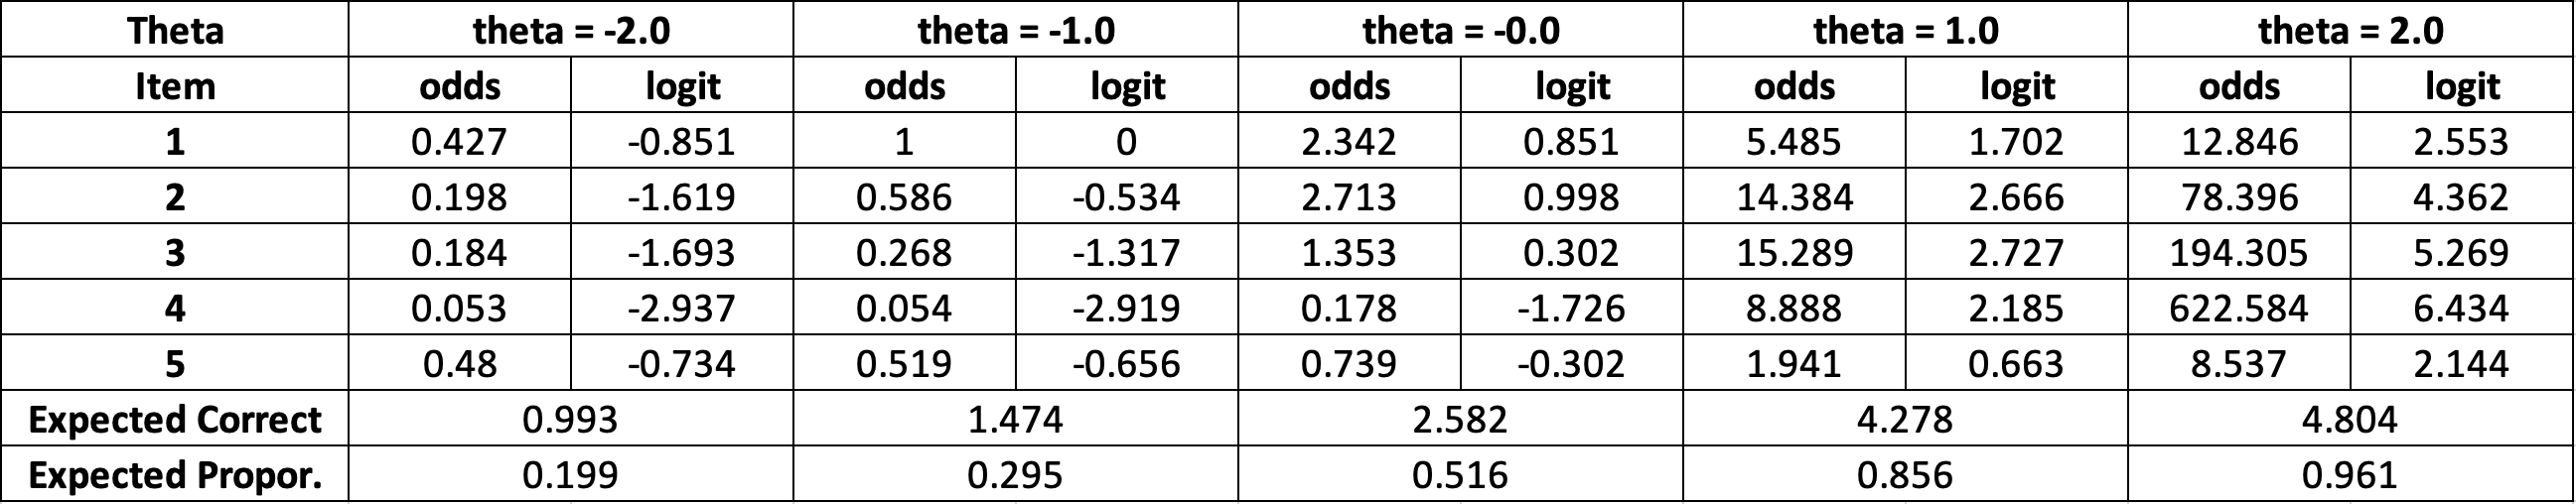
\includegraphics{table_1.png}

\end{document}
